\section{Идеи для fix-up'ов} % device
\subtitle{От сотворения мира в звёздном храме до тепловой смерти Вселенной}
\begin{epigraph}
    Welcome to my nightmare
    \flushright{\normalfont Alice Cooper, март~1975}
\end{epigraph}
\begin{flushleft}\parskip1em
    Классический (инверсивный) пример: ночь -- это день, день -- это ночь.

    Календарь:
    \begin{itemize}
        \item по обращению комет вокруг Солнца;
        \item по обращению Солнца вокруг центра галактики;
        \item персональный календарь по биоритмам человека/ его кота/собаки...
        \item По сообщениям об открытии новой экзопланеты.
    \end{itemize}

    Календарь для людей творческих профессий -- от вдохновения до запоя.

    Календарь для весёлых наркоманов -- генератор случайных чисел.

    Календарь трудо- и алкоголика -- от получки до получки.

    Лунный календарь для дачников и соннамбул.

    Календарь основанный на выходе новинок apple/windows и прочих техногигантов.

    Квазипериодические хронометры (следим за их колебаниями):
    \begin{itemize}
        \item Бревно на волнах.
        \item Качелька на ветру.
        \item Космический парус на солнечном ветру.
        \item Датчик движения на крыле стрижа.
        \item Удары молний в кдиную сеть громоотводов (её нужно создать) по всей планете.
        \item По концентрации пыли в помещении (+нужно создать соответствующий прибор для её оценки).
        \item для автолюбителей и вообще техников: по промежуткам между очередной поломкой приборов.
        \item для медиков и вирусологов: от эпидемии до эпидемии.
    \end{itemize}

    \begin{figure}[ht!]
        \centering
        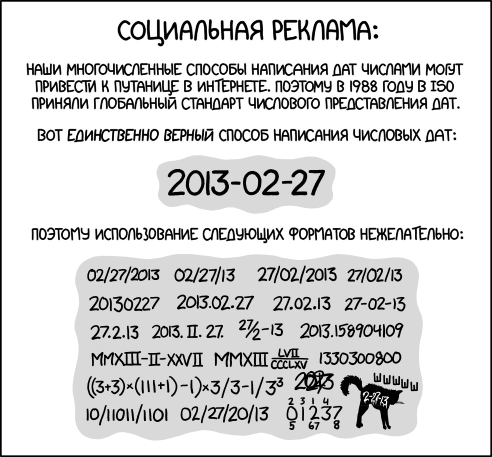
\includegraphics[width=0.6\textwidth]{xkcd-iso-8601}
    \end{figure}

    Специфические хронометры:
    \begin{itemize}
        \item Колебательный контур с током при \( T \to 0 K \).
        \item На реакции Белоусова--Жаботинского.
        \item На пульсации пульсаров/двойных звёзд.
    \end{itemize}

    Способы записи времени:
    \begin{itemize}
        \item через молекулы ДНК.
        \item С помощью круговых диаграмм и процентов оставшейся части светового дня.
        \item через прогрессию арифметическую/геометрическую.
        \item через фракталы.
        \item через мелодии и звуки.
    \end{itemize}

    Разное:
    \begin{enumerate}
        \item Использовать древние календари различных минувших цивилизаций.
        \item Использовать современные календари, но с мёртвыми языками.
        \item Вести календарь не с начала месяца/года/тысячелетия, а с конца:\\
            20/09/2016 = 10/04/2984
        \item Вести календарь по солнечным и лунным затмениям.
        \item по приливам и отливам.
        \item по периоду полураспада.
        \item по цифрам числа \( \pi \), \( e \), \( \hbar \):\\
            03/14/15\qquad 02/71/82\qquad 01/05/45
        \item использовать отсчёт как в unix системах
        \item считать в минутах, часах, ...
        \item записывать время в виде/через/с помощью: функции, тензора, алгоритма, группы, кольца, графа/дерева, 
            предиката, цикла, числа Фибоначчи, числа Каталана, ОДУ и ДУЧП, через количество пикселей на 
            определённых картинках -- каждому месяцу -- каринка -- число пикселей -- дни, ...
        \item использовать необычную форму записи\\
            10+4+3+2/4+3+2/10+4+2\qquad \#\#\#\#=-:\#\#-:\#\#\#\#
        \item Измерять время с помощью дождя: выбираем площадку фиксированного размера, и считаем за промежутки времени ---
        между последовательным падением капель на неё. Проводим усреднения по площадкам, времени, интенсивности дождя
        и т.д. для вычисления эталона.
    \end{enumerate}
\end{flushleft}

\begin{figure}[ht!]
    \centering
    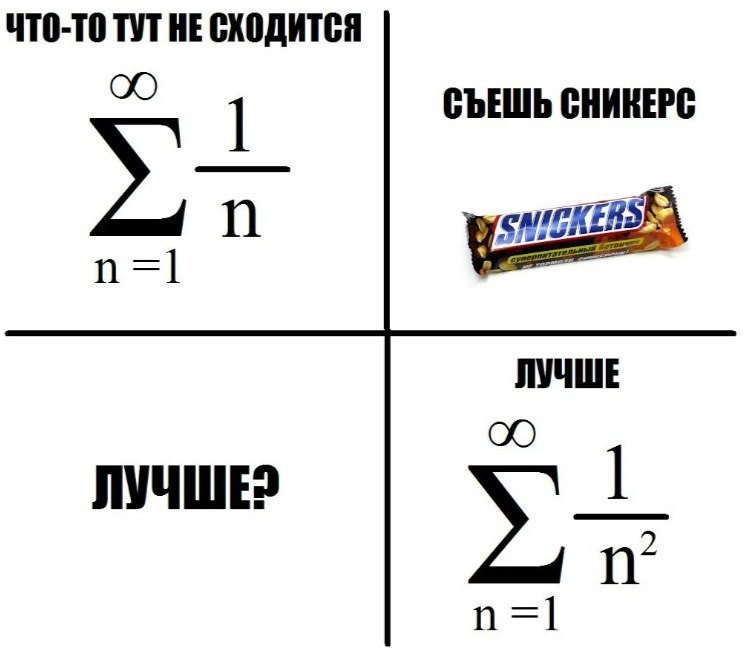
\includegraphics[width=\textwidth]{snickers}
\end{figure}
